\section{Verification battery}
\label{sec:verification}

\texttt{verification.py} implements the checks not already covered by each
module's own unit tests.

\paragraph{Protected-option sweep.} Across all three scheduled resets, four
maturity fractions each, and an independent four-point $u$-mesh (48
combinations, not a single probe), $|\Phi_{\rm before}-\Phi_{\rm after}|$ for
$T<t_n$ is reported in Table~\ref{tab:verification-summary} -- machine-precision
zero, confirming Theorem \texttt{thm:bcrc-reserve}'s reset-preservation
claim exactly, for exactly the options it protects (options settling before
the reset). Options with $T>t_n$ are \emph{not} protected and do move under
recalibration, by design (Fig.~\ref{fig:reset-invariance}).

\paragraph{Negative control.} \texttt{uncompensated\_transform} removes the
reserve/envelope machinery and prices directly off $p_n$. It VIOLATES the
same protected-option invariance the real construction satisfies exactly,
by three orders of magnitude (Table~\ref{tab:verification-summary}) --
confirming the sweep has statistical/analytical power and the reserve
mechanism is load-bearing, not a vacuous formality.

\paragraph{Off-grid generator residual.} $d/dT\log\Phi_t(u,T)$, computed two
independent ways (central finite difference in $T$ vs.\ the analytic RHS
assembled from the Riccati ODE + current jump exponent + $\ell_T(u)$), agree
at maturities chosen to coincide with neither a reset time nor a scheduled
model expiry, at every state -- the closest available analogue, for this
transform-based construction, to \texttt{cor:bates-offgrid-drift}'s
backward-generator identity.

\paragraph{Chain composition.} $P(\tau_1)P(\tau_2)=P(\tau_1+\tau_2)$ (Chapman--Kolmogorov)
checked directly on the $X$-chain's \texttt{expm}-based transition matrix.

\paragraph{Convergence under refinement.} \texttt{quadrature\_refinement\_convergence}
confirms the reserve integral's Gauss--Legendre quadrature error decreases
monotonically as $n_{\rm quad}$ increases (25 up to 800 nodes), rather than
merely agreeing with itself at one fixed order.

\paragraph{Monte Carlo, with confidence interval, not treated as proof.}
The independent MC pricing check (Sec.~\ref{sec:continuation-transform})
is reported with its Monte Carlo standard error explicitly
(Table~\ref{tab:verification-summary}); non-rejection within $6$ standard
errors is reported as exactly that, not as a proof of correctness -- the
proofs are the analytic checks above and in Sec.~\ref{sec:reserve}.

\begin{table}[H]
\centering
\begin{tabular}{lr}
\toprule
Check & Result \\
\midrule
Protected-option sweep, max $|\Phi_{\rm before}-\Phi_{\rm after}|$ & $4.34e-19$ \\
Protected-option sweep, combinations tested & 48 \\
Negative control, max $|\Phi_{\rm before}-\Phi_{\rm after}|$ & $7.65e-05$ \\
Negative control fails as expected & Yes \\
Independent MC: Fourier price ($K=1$, $T=t_1$) & $0.008309$ \\
Independent MC: MC price $\pm$ 1 s.e. & $0.008284 \pm 0.000041$ \\
Independent MC: $|$diff$|$ within 6 s.e. & Yes \\
Independent MC: seed, $n_{\rm paths}$ & 7, 400,000 \\
\bottomrule
\end{tabular}

\caption{Verification battery summary. See \texttt{data/verification\_summary.json}
for the full machine-readable record.}
\label{tab:verification-summary}
\end{table}

\begin{figure}[H]
\centering
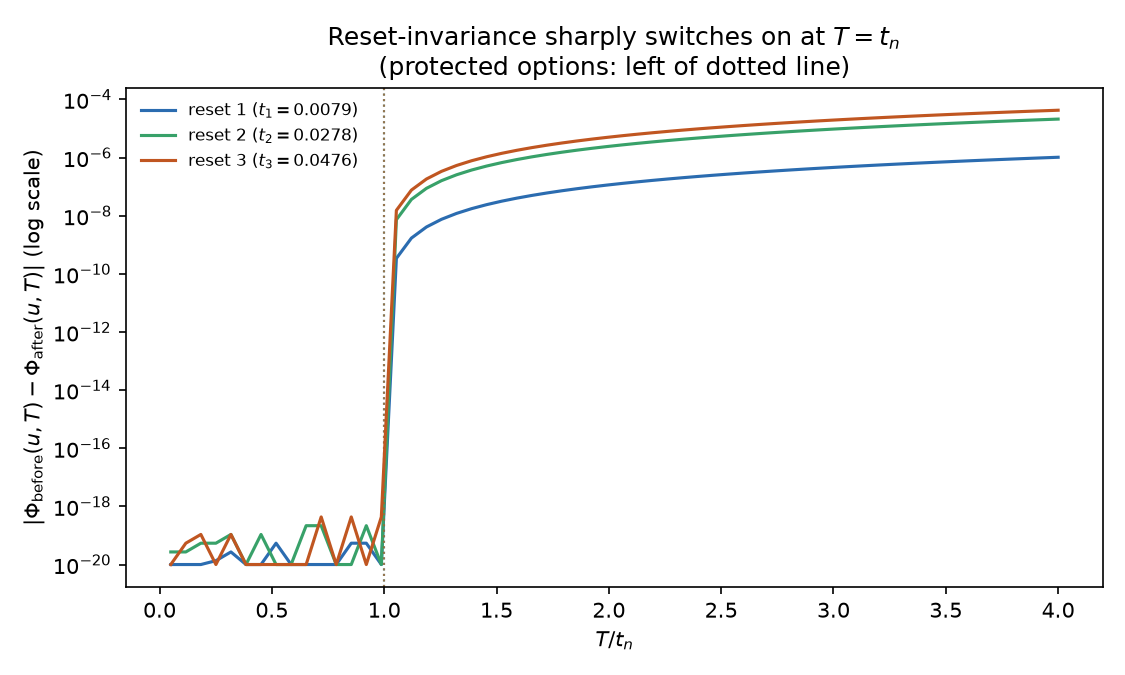
\includegraphics[width=0.75\textwidth]{figures/reset_invariance_by_maturity.png}
\caption{$|\Phi_{\rm before}(u,T)-\Phi_{\rm after}(u,T)|$ vs.\ $T/t_n$ for
each of the three resets: exactly zero (floating-point noise) for
$T<t_n$ (protected), nonzero and growing for $T>t_n$ (unprotected, moves
by design under recalibration).}
\label{fig:reset-invariance}
\end{figure}
